% !TeX program = xelatex
\documentclass[12pt]{article}
\usepackage[a0paper,portrait,margin=16mm]{geometry}
\usepackage{fontspec,graphicx,booktabs,array,ragged2e,amsmath,amssymb}
\usepackage[most]{tcolorbox}
\usepackage{xcolor,tikz,microtype}
\usetikzlibrary{arrows.meta,positioning}
\graphicspath{{assets/}{./}}
\setsansfont{TeX Gyre Heros}\setmainfont{TeX Gyre Heros}
\renewcommand{\familydefault}{\sfdefault}\pagestyle{empty}
\setlength{\parindent}{0pt}\setlength{\parskip}{3.8mm}
\setlength{\tabcolsep}{2.4mm}\renewcommand{\arraystretch}{1.26}
\definecolor{Burgundy}{HTML}{841B20}\definecolor{BurgundyDark}{HTML}{5B1015}
\definecolor{BurgundyMid}{HTML}{A5474C}\definecolor{Rose}{HTML}{F2E3E4}
\definecolor{RoseDeep}{HTML}{E3C8CA}\definecolor{Ivory}{HTML}{FBF8F6}
\definecolor{Ink}{HTML}{241D1E}\definecolor{Rule}{HTML}{D8C9CA}
\definecolor{NoteGray}{HTML}{F0EEEE}\definecolor{NoteInk}{HTML}{655F60}
\pagecolor{Ivory}\color{Ink}
\newcommand{\TitleFont}{\fontsize{59}{65}\selectfont\bfseries}
\newcommand{\AuthorFont}{\fontsize{29}{35}\selectfont}
\newcommand{\AffilFont}{\fontsize{25}{30}\selectfont}
\newcommand{\BodyFont}{\fontsize{32.5}{41}\selectfont}
\newcommand{\SmallFont}{\fontsize{25}{32}\selectfont}
\newcommand{\best}[1]{\textbf{\color{Burgundy}#1}}
\newtcolorbox{posterblock}[2][]{enhanced,colback=white,colframe=Rule,boxrule=.8mm,
 arc=5mm,left=8mm,right=8mm,top=6mm,bottom=6mm,title={#2},coltitle=white,
 colbacktitle=Burgundy,fonttitle=\fontsize{36}{43}\selectfont\bfseries,
 boxed title style={arc=4mm,boxrule=0pt},attach boxed title to top left={xshift=0mm,yshift=-1mm},
 before upper={\BodyFont\RaggedRight},#1}
\newtcolorbox{softpanel}[1][]{enhanced,colback=Rose,colframe=BurgundyMid,boxrule=.7mm,
 arc=4mm,left=7mm,right=7mm,top=5mm,bottom=5mm,before upper={\BodyFont\RaggedRight},#1}
\newtcolorbox{notepanel}[1][]{enhanced,colback=NoteGray,colframe=Rule,boxrule=.6mm,
 arc=4mm,left=8mm,right=8mm,top=4mm,bottom=4mm,
 before upper={\color{NoteInk}\fontsize{25}{32}\selectfont\RaggedRight},#1}
\newcommand{\vgap}{\vspace{6mm}}
\newcommand{\pill}[1]{\tikz[baseline=(x.base)]\node[fill=Rose,draw=BurgundyMid,
 rounded corners=3mm,inner xsep=4mm,inner ysep=2mm,text=BurgundyDark,
 font=\bfseries\fontsize{21}{26}\selectfont](x){#1};}
\newcommand{\heropill}[1]{\tikz[baseline=(x.base)]\node[fill=Rose,draw=BurgundyMid,
 rounded corners=4mm,line width=.8mm,inner xsep=7mm,inner ysep=3.5mm,text=BurgundyDark,
 font=\bfseries\fontsize{27}{33}\selectfont](x){#1};}
\begin{document}
\begin{tcolorbox}[enhanced,colback=BurgundyDark,colframe=BurgundyDark,arc=7mm,
 boxrule=0pt,left=11mm,right=11mm,top=8mm,bottom=8mm]
\begin{minipage}[c]{.12\textwidth}\centering
 \begin{tikzpicture}\clip (0,0) circle (39mm);
 \node[inner sep=0pt] at (0,0){
\includegraphics[width=78mm]{xju_logo.jpg}};\end{tikzpicture}
\end{minipage}\hfill
\begin{minipage}[c]{.72\textwidth}\centering\color{white}
 {\TitleFont DualFaith at NLPCC-2026 Task 10:\\[2mm]Faithfulness Verification for Scientific Reports}\par
 \vspace{6mm}{\AuthorFont Wenbiao Zhao$^{1,\dagger}$ \quad Longkun Shi$^{1,\dagger}$ \quad
 Zicheng Zuo$^{1,2,3}$ \quad Turdi Tohti$^{1,2,3,*}$}\par
 \vspace{3mm}{\AffilFont
 $^1$School of Computer Science and Technology, Xinjiang University\\
 $^2$Joint International Research Laboratory of Silk Road Multilingual Cognitive Computing\\
 $^3$Xinjiang Key Laboratory of Signal Detection and Processing\\
 $^\dagger$Equal contribution \quad $^*$Corresponding author}
\end{minipage}\hfill
\begin{minipage}[c]{.12\textwidth}\centering
 
\includegraphics[height=61mm]{nlpcc_macau_mark.png}\par\vspace{1mm}
 {\color{white}\fontsize{27}{31}\selectfont\bfseries NLPCC 2026}\par
 {\color{RoseDeep}\fontsize{16}{20}\selectfont Macau, China}
\end{minipage}\end{tcolorbox}
\vspace{7mm}
\begin{posterblock}[colframe=BurgundyMid,boxrule=1.1mm]{Why Scientific Faithfulness Needs Two Kinds of Evidence}
\begin{minipage}[c]{.72\linewidth}
AI-assisted scientific writing must be fluent \emph{and} grounded. A results sentence may misread a figure, invent an entity, assert an unsupported mechanism, or overgeneralize a local result. A related-work claim may cite a topically relevant paper that does not actually support it. \textbf{DualFaith} addresses both failure modes with task-specific evidence modeling.
\end{minipage}\hfill
\begin{minipage}[c]{.26\linewidth}\centering
 \heropill{Track 1: figures \& tables}\par\vspace{6mm}\heropill{Track 2: cited full text}
\end{minipage}\end{posterblock}
\vspace{7mm}
\noindent\begin{minipage}[t]{.49\textwidth}\vspace{0pt}
\begin{posterblock}[colframe=Burgundy,boxrule=1.2mm]{Track 1: Multimodal Sentence Verification}
 \centering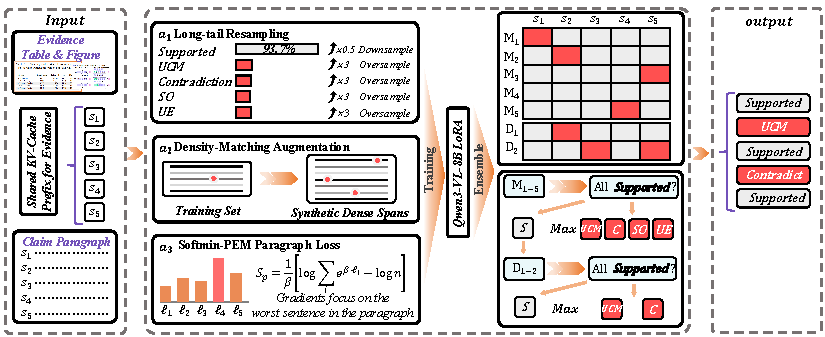
\includegraphics[width=\linewidth]{track1_figure.pdf}
 \vspace{4mm}\RaggedRight
 Each sentence is assigned one of five labels using its claim paragraph, caption, and rendered figure/table. Qwen3-VL-8B-Instruct is adapted with LoRA; the vision tower remains frozen.
 \begin{softpanel}\textbf{Recall-additive ensemble.} Five heterogeneous members form a minority-label union. Two density-augmented members can add only causal/mechanistic or contradiction labels to positions still predicted as Supported. This directly targets the paragraph exact-match bottleneck.\end{softpanel}
 \centering\pill{LoRA $r=16,\ \alpha=32$}\quad\pill{softmin-PEM}\quad\pill{long-tail resampling}
\end{posterblock}
\vspace{13mm}
\begin{posterblock}{Track 1: Data and Metric Insight}
 \textbf{Severe imbalance:} 16,438 of 17,547 train--development sentences (93.7\%) are Supported; all four minority classes total only 6.3\%.

 Only 0.46\% of training paragraphs with at least six sentences contain two or more minority sentences, while approximately 84\% of Phase-1 test paragraphs contain at least one. The all-Supported baseline therefore falls to 18.85.
 \begin{softpanel}The official score averages sentence-level Macro-F1 and paragraph exact match (PEM). Missing one minority sentence invalidates the whole paragraph, so \textbf{minority recall—not suppression—is the central Track-1 bottleneck}.\end{softpanel}
\end{posterblock}
\vspace{13mm}
\begin{posterblock}[bottom=8mm,
 overlay unbroken={\node[anchor=south east,fill=BurgundyDark,text=white,
 rounded corners=3mm,inner xsep=5mm,inner ysep=2.4mm,
 font=\bfseries\fontsize{21}{25}\selectfont]
 at ([xshift=-4mm,yshift=4mm]frame.south east){Second of 11 teams};}]
 {Track 1: Official Result and Sensitivity}
\noindent\begin{minipage}[t]{.43\linewidth}\vspace{0pt}\centering{\fontsize{20.5}{26}\selectfont
\begin{tabular}{@{}lrrr@{}}\toprule
System & Final & Phase 1 & Phase 2\\\midrule
SUAT-NLP & \best{68.90} & \best{51.85} & 85.95\\
\textbf{DualFaith} & 68.79 & 50.61 & \best{86.97}\\
BIT-TrustAI & 57.99 & 44.09 & 71.88\\
ZZUNLP\_Han & 55.47 & 42.44 & 68.50\\
YNU-HPCC & 46.16 & 31.93 & 60.39\\\bottomrule
\end{tabular}}\end{minipage}\hfill
\begin{minipage}[t]{.54\linewidth}\vspace{0pt}\centering{\fontsize{20.5}{26}\selectfont
\begin{tabular}{@{}lrr@{}}\toprule
Phase-1 setting & Score & Minority predictions\\\midrule
Near-all Supported & 18.85 & 46\\Best single member & 47.80 & 253\\
Union of 3 members & 48.22 & 339\\Union of 5 members & 50.26 & 382\\
\textbf{Final density-augmented union} & \best{50.61} & \best{399}\\\bottomrule
\end{tabular}}\end{minipage}
\par\vspace{5mm}\RaggedRight
Only 0.11 points behind first overall; best Phase-2 score among the top five and highest Phase-1 Macro-F1 (57.54).
\end{posterblock}
\end{minipage}\hfill
\begin{minipage}[t]{.49\textwidth}\vspace{0pt}
\begin{posterblock}[colframe=Burgundy,boxrule=1.2mm]{Track 2: Citation Support with Frozen Evidence}
 \centering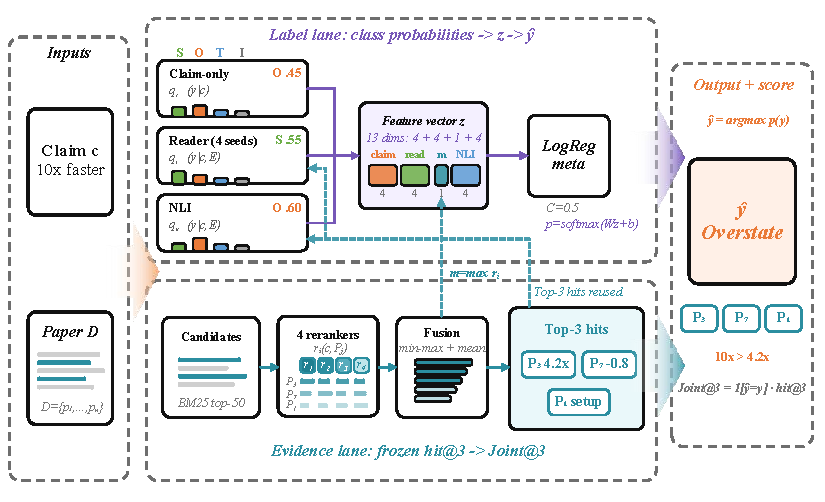
\includegraphics[width=.90\linewidth]{track2_figure.pdf}\par
 \vspace{4mm}\RaggedRight
 BM25 retrieves candidates; two DeBERTa cross-encoders, MonoT5-large, and frozen Qwen3-Reranker-4B are normalized per record and equally fused into a \textbf{fixed top-three evidence list}.
 \begin{softpanel}\textbf{Domain-robust label stacking.} A four-seed DeBERTa evidence reader, a claim-only classifier, a frozen multi-task NLI posterior, and the maximum evidence score feed a logistic-regression meta-classifier. Freezing retrieval isolates label calibration from evidence uncertainty.\end{softpanel}
 \centering\pill{4-way label}\quad\pill{top-3 evidence}\quad\pill{stacked posteriors}
\end{posterblock}
\vspace{13mm}
\begin{posterblock}{Track 2: Domain Shift and Metric Coupling}
 Phase 1 is dominated by physics/materials (64.8\%), while train--development (49.3\%) and Phase 2 (52.8\%) are CS/AI/ML-heavy. A topic-holdout probe loses about 7 Macro-F1 points for the evidence reader but only 2 for the claim-only model.
 \begin{softpanel}Joint@3 succeeds only when the label is correct \emph{and} a gold paragraph appears in the retrieved top three. Strong classification without matching evidence is insufficient; stable evidence plus robust label correction wins under shift.\end{softpanel}
\end{posterblock}
\vspace{13mm}
\begin{posterblock}[bottom=8mm,
 overlay unbroken={\node[anchor=south east,fill=BurgundyDark,text=white,
 rounded corners=3mm,inner xsep=5mm,inner ysep=2.4mm,
 font=\bfseries\fontsize{21}{25}\selectfont]
 at ([xshift=-4mm,yshift=4mm]frame.south east){First of 15 teams};}]
 {Track 2: Official Result and Ablation}
\noindent\begin{minipage}[t]{.53\linewidth}\vspace{0pt}\centering{\fontsize{20.5}{26}\selectfont
\begin{tabular}{@{}lrrrr@{}}\toprule
System & Final & Macro-F1 & Joint@3 & Phase 2\\\midrule
\textbf{DualFaith} & \best{86.27} & 91.18 & \best{81.37} & \best{86.33}\\
Lenormand & 82.99 & 89.55 & 76.43 & 84.70\\
HER-DAC & 81.61 & 93.05 & 70.16 & 81.52\\
ZZUNLP\_Han & 81.38 & \best{94.25} & 68.51 & 81.88\\
SUAT-NLP & 79.01 & 91.02 & 67.00 & 77.13\\\bottomrule
\end{tabular}}\end{minipage}\hfill
\begin{minipage}[t]{.44\linewidth}\vspace{0pt}\centering{\fontsize{20.5}{26}\selectfont
\begin{tabular}{@{}lrrr@{}}\toprule
Phase-1 label system & Score & Macro-F1 & Joint@3\\\midrule
Four-seed reader & 83.10 & 87.02 & 79.19\\
$+$ claim-only mixture & 85.10 & 89.41 & 80.79\\
$+$ NLI + meta-classifier & \best{86.21} & \best{90.46} & \best{81.96}\\\bottomrule
\end{tabular}}\end{minipage}
\par\vspace{5mm}\RaggedRight
A 3.28-point lead over second place. Phase 1 and blind Phase 2 differ by only 0.12, demonstrating stability across the domain shift.
\end{posterblock}
\end{minipage}
\vspace{4mm}
\begin{posterblock}{Transferable Lessons}
\begin{minipage}[t]{.48\linewidth}
\textbf{Track 1: align with error density.} Higher image resolution, extra epochs, supervised chain-of-thought, OCR, and suppression rules did not yield consistent gains. Diverse union members recover complementary minority cases.
\end{minipage}\hfill
\begin{minipage}[t]{.48\linewidth}
\textbf{Track 2: decouple retrieval and labeling.} Domain-adaptive/adversarial training, label-shift correction, extra rerankers, and eight reader seeds failed selection. Fixing evidence lets label-side signals correct domain-sensitive errors safely.
\end{minipage}\end{posterblock}
\vspace{5mm}
\begin{notepanel}
\begin{minipage}[t]{.34\linewidth}
\textbf{ABSTRACT IN BRIEF}\par
DualFaith verifies whether scientific statements are supported by experimental figures and tables or by cited papers. Track 1 labels every sentence of a results paragraph against its figure; Track 2 labels an atomic claim against the cited paper and returns the supporting paragraphs. Both pipelines pair minority-recall ensembling with frozen evidence retrieval and domain-robust label stacking.
\end{minipage}\hfill
\begin{minipage}[t]{.26\linewidth}
\textbf{LIMITATIONS}\par
Track 1 includes partial recipe reconstruction and PEM nondeterminism. Track 2 may inherit stylistic cues from claim-only modeling, and its development set contains only 433 records. Broader evaluation on human-written claims remains future work.
\end{minipage}\hfill
\begin{minipage}[t]{.18\linewidth}
\textbf{ACKNOWLEDGMENTS}\par
Funded by the Xinjiang Talent Development Fund (Grant No. XJRC-2025-KJ-PY-KJLJ-051). We thank the NLPCC-2026 Task 10 organizers and evaluators.
\end{minipage}\hfill
\begin{minipage}[t]{.14\linewidth}\centering\vspace{0pt}

\includegraphics[height=68mm]{qr-talk.png}
\end{minipage}
\end{notepanel}
\vfill
\begin{tcolorbox}[enhanced,colback=Burgundy,colframe=Burgundy,boxrule=0pt,arc=6mm,left=11mm,right=11mm,top=7mm,bottom=7mm]
\begin{minipage}[c]{.75\textwidth}
{\color{RoseDeep}\fontsize{19}{23}\selectfont\bfseries TAKEAWAY}\par\vspace{1mm}
{\color{white}\fontsize{27}{33}\selectfont\bfseries Faithfulness verification improves when the system is designed around the metric and the shift: add minority recall for multimodal claims, and freeze evidence before robust citation-label stacking.}
\end{minipage}\hfill
\begin{minipage}[c]{.22\textwidth}\RaggedLeft\color{white}
{\fontsize{21}{25}\selectfont\bfseries Contact}\par
{\fontsize{18}{22}\selectfont turdy@xju.edu.cn}\par
{\fontsize{15}{19}\selectfont Xinjiang University}
\end{minipage}\end{tcolorbox}
\end{document}
